\section*{7.2 Distribuições a Priori e a Posteriori}
A distribuição de um parâmetro antes da observação de quaisquer dados é chamada de distribuição \textit{a priori}. A distribuição condicional do parâmetro, dados os valores observados, é chamada de distribuição \textit{a posteriori}. Se inserirmos os valores observados dos dados na f.d.p. (função de densidade de probabilidade) ou f.p. (função de probabilidade) condicional, e considerarmos o resultado como uma função apenas do parâmetro, o resultado é chamado de função de \textit{verossimilhança}.

\subsection*{A Distribuição a Priori}

\noindent\textbf{Exemplo 7.2.1} \quad \textbf{Tempo de Vida de Componentes Eletrônicos.} No Exemplo 7.1.1, os tempos de vida $X_1, X_2, \dots$ de componentes eletrônicos foram modelados como variáveis aleatórias i.i.d. exponenciais com parâmetro $\theta$ condicional a $\theta$, e $\theta$ foi interpretado como a taxa de falha dos componentes. Notamos que $n/\sum_{i=1}^{n}X_i$ deveria convergir em probabilidade para $\theta$ quando $n \to \infty$. Dissemos então que $\theta$ tinha a distribuição gama com parâmetros 1 e 2.

A distribuição de $\theta$ mencionada no final do Exemplo 7.2.1 foi atribuída antes de se observar a vida útil de qualquer componente. Por essa razão, chamamos isso de \textit{distribuição a priori}.

\vspace{1cm}
\noindent\textbf{Definição 7.2.1} \quad \textbf{Distribuição a Priori/f.p./f.d.p.} Suponha que se tenha um modelo estatístico com parâmetro $\theta$. Se trata $\theta$ como uma variável aleatória, então a distribuição que se atribui a $\theta$ antes de observar quaisquer outras variáveis aleatórias de interesse é chamada de sua \textit{distribuição a priori}. Se o espaço de parâmetros for no máximo contável, então a distribuição a priori é discreta e sua f.p. é chamada de \textit{f.p. a priori} de $\theta$. Se a distribuição a priori for contínua, então sua f.d.p. é chamada de \textit{f.d.p. a priori} de $\theta$. Usaremos comumente o símbolo $\xi(\theta)$ para denotar a f.p. ou f.d.p. a priori de $\theta$.

\vspace{1cm}
Quando se trata um parâmetro como uma variável aleatória, o nome ``distribuição a priori'' é meramente outro nome para a distribuição marginal do parâmetro.

\vspace{1cm}
\noindent\textbf{Exemplo 7.2.2} \quad \textbf{Moeda Justa ou de Duas Caras.} Seja $\theta$ a probabilidade de obter uma cara quando uma certa moeda é lançada, e suponha que se saiba que a moeda é justa ou tem cara em ambos os lados. Portanto, os únicos valores possíveis de $\theta$ são $\theta=1/2$ e $\theta=1$. Se a probabilidade a priori de que a moeda é justa for 0.8, então a f.p. a priori de $\theta$ é $\xi(1/2)=0.8$ e $\xi(1)=0.2$.

\vspace{1cm}
\noindent\textbf{Exemplo 7.2.3} \quad \textbf{Proporção de Itens Defeituosos.} Suponha que a proporção $\theta$ de itens defeituosos em um grande lote manufaturado seja desconhecida e que a distribuição a priori atribuída a $\theta$ seja a distribuição uniforme no intervalo $[0, 1]$. Então a f.d.p. a priori de $\theta$ é
\begin{equation}
\xi(\theta) = 
\begin{cases}
1 & \text{para } 0 < \theta < 1, \\
0 & \text{caso contrário.}
\end{cases}
\tag{7.2.1}
\end{equation}

A distribuição a priori de um parâmetro $\theta$ deve ser uma distribuição de probabilidade sobre o espaço de parâmetros $\Omega$. Assumimos que o experimentador ou estatístico será capaz de resumir seu conhecimento prévio e crenças sobre onde o valor de $\theta$ provavelmente se encontra em $\Omega$ na forma de uma distribuição a priori para $\theta$. Ou seja, antes que os dados experimentais tenham sido coletados ou observados, a experiência e o conhecimento passados do experimentador o levarão a acreditar que $\theta$ tem maior probabilidade de estar em certas regiões de $\Omega$ do que em outras. Assumiremos que as verossimilhanças relativas das diferentes regiões podem ser expressas em termos de uma distribuição de probabilidade em $\Omega$, ou seja, a distribuição a priori de $\theta$.

\vspace{1cm}
\noindent\textbf{Exemplo 7.2.4} \quad \textbf{Tempo de Vida de Lâmpadas Fluorescentes.} Suponha que os tempos de vida (em horas) de lâmpadas fluorescentes de um certo tipo devam ser observados e que o tempo de vida de qualquer lâmpada em particular tenha a distribuição exponencial com parâmetro $\theta$. Suponha também que o valor exato de $\theta$ seja desconhecido, e com base na experiência prévia, a distribuição a priori de $\theta$ seja considerada a distribuição gama para a qual a média é 0.0002 e o desvio padrão é 0.0001. Determinaremos a f.d.p. a priori de $\theta$.
Suponha que a distribuição a priori de $\theta$ seja a distribuição gama com parâmetros $\alpha_0$ e $\beta_0$. Foi mostrado no Teorema 5.7.4 que a média desta distribuição é $\alpha_0/\beta_0$ e a variância é $\alpha_0/\beta_0^2$. Portanto, $\alpha_0/\beta_0 = 0.0002$ e $\alpha_0/\beta_0^2 = (0.0001)^2$. Essas duas equações resultam em $\alpha_0=4$ e $\beta_0=20.000$. Segue-se de Eq. (5.7.13) que a f.d.p. a priori de $\theta$ para $\theta > 0$ é a seguinte:
\begin{equation}
\xi(\theta) = \frac{(20.000)^4}{3!} \theta^3 e^{-20.000\theta}. \tag{7.2.2}
\end{equation}
Além disso, $\xi(\theta)=0$ para $\theta \le 0$.

\vspace{1cm}
No restante desta seção e nas Seções 7.3 e 7.4, focaremos em problemas de inferência estatística nos quais o parâmetro $\theta$ é uma variável aleatória e, portanto, precisa ter uma distribuição atribuída. Referir-nos-emos à distribuição indexada por $\theta$ para as outras variáveis aleatórias de interesse como a distribuição condicional para essas variáveis aleatórias dado $\theta$. Esta é precisamente a linguagem usada no Exemplo 7.2.1 onde o parâmetro é $\theta$, a taxa de falha. Referindo-se à f.p. ou f.d.p. condicional de variáveis aleatórias condicionais e suas f.p.s e f.d.p.s. não condicionais, usaremos a notação da Seção 7.2.1. Por exemplo, se seja $\mathbf{X}=(X_1, \dots, X_m)$ no Exemplo 7.2.1, a f.d.p. condicional de $\mathbf{X}$ dado $\theta$ é
\begin{equation}
f_m(\mathbf{x}|\theta) = 
\begin{cases}
\theta^m \exp(-\theta[x_1 + \dots + x_m]) & \text{para todos } x_i > 0, \\
0 & \text{caso contrário}.
\end{cases}
\tag{7.2.3}
\end{equation}

Em muitos problemas, como no Exemplo 7.2.1, os dados observáveis $X_1, X_2, \dots$ são modelados como uma amostra aleatória de uma distribuição univariada indexada por $\theta$. Nestes casos, seja $f(x|\theta)$ a f.p. ou f.d.p. de uma única variável aleatória sob a distribuição indexada por $\theta$. Em tal caso, usando a notação acima,
$$ f_m(\mathbf{x}|\theta) = f(x_1|\theta) \cdots f(x_m|\theta). $$
Quando tratamos $\theta$ como uma variável aleatória, $f(x_i|\theta)$ é a f.p. ou f.d.p. condicional de cada observação $X_i$ dado $\theta$, e as observações são condicionalmente i.i.d. dado $\theta$. Em resumo, as duas expressões a seguir devem ser entendidas como equivalentes:
\begin{itemize}
    \item $X_1, \dots, X_n$ formam uma amostra aleatória com f.p. ou f.d.p. $f(x|\theta)$.
    \item $X_1, \dots, X_n$ são condicionalmente i.i.d. dado $\theta$ com f.p. ou f.d.p. condicional $f(x|\theta)$.
\end{itemize}
Embora geralmente usemos a primeira expressão por simplicidade, é frequente que a segunda expressão seja útil para lembrar que as duas expressões são equivalentes quando tratamos $\theta$ como uma variável aleatória.

\subsection*{Análise de Sensibilidade e Prioris Impróprias}

No Exemplo 2.3.8 na página 84, vimos uma situação em que dois conjuntos muito diferentes de probabilidades a priori foram usados para uma coleção de eventos. Após a observação dos dados, no entanto, as probabilidades a posteriori eram bastante semelhantes. No Exemplo 5.8.4 na página 330, usamos uma grande coleção de distribuições a priori para a probabilidade de um parâmetro a fim de ver o quanto o impacto de uma distribuição a priori sobre a probabilidade a posteriori de um único evento importante. É uma prática comum comparar as distribuições a posteriori que surgem de várias distribuições a priori diferentes para ver o quanto o efeito da distribuição a priori tem sobre as respostas a questões importantes. Tais comparações são chamadas de \textit{análise de sensibilidade}.

É muito comum o caso de que diferentes distribuições a priori não fazem muita diferença depois que os dados foram observados. Isso é especialmente verdadeiro se houver muitos dados ou se as distribuições a priori que estão sendo comparadas são muito dispersas. Essa observação tem duas implicações importantes. Primeiro, o fato de que diferentes experimentadores podem não concordar sobre uma distribuição a priori torna-se menos importante se houver muitos dados. Segundo, os experimentadores podem estar menos inclinados a gastar tempo especificando uma distribuição a priori se não for fazer muita diferença qual deles é especificado. Infelizmente, se não se especifica alguma distribuição a priori, não há como calcular uma distribuição condicional do parâmetro dados os dados.

Como um expediente, existem alguns cálculos disponíveis que tentam capturar a ideia de que os dados contêm muito mais informações do que as disponíveis a priori. Geralmente, esses cálculos envolvem o uso de uma função $\xi(\theta)$ como se fosse uma f.d.p. a priori para o parâmetro $\theta$, mas tal que $\int\xi(\theta)d\theta = \infty$, o que viola claramente a definição de f.d.p. Tais prioris são chamadas de \textit{impróprias}. Discutiremos prioris impróprias mais detalhadamente na Seção 7.3.

\subsection*{A Distribuição a Posteriori}

\noindent\textbf{Exemplo 7.2.5} \quad \textbf{Tempo de Vida de Lâmpadas Fluorescentes.} No Exemplo 7.2.4, construímos uma distribuição a priori para o parâmetro $\theta$ que especifica a distribuição exponencial para uma coleção de tempos de vida de lâmpadas fluorescentes. Suponha que observemos uma coleção de $n$ tais tempos de vida. Como mudaríamos a distribuição de $\theta$ para levar em conta os dados observados?

\vspace{1cm}
\noindent\textbf{Definição 7.2.2} \quad \textbf{Distribuição/f.p./f.d.p. a Posteriori.} Considere um problema de inferência estatística com parâmetro $\theta$ e variáveis aleatórias $X_1, \dots, X_n$, a serem observadas. A distribuição condicional de $\theta$ dados $X_1, \dots, X_n$ é chamada de \textit{distribuição a posteriori} de $\theta$. A f.p. ou f.d.p. condicional de $\theta$ dados $X_1=x_1, \dots, X_n=x_n$ é chamada de \textit{f.p. a posteriori} ou \textit{f.d.p. a posteriori} de $\theta$ e é tipicamente denotada por $\xi(\theta|x_1, \dots, x_n)$.

\vspace{1cm}
Quando se trata o parâmetro como uma variável aleatória, o nome ``distribuição a posteriori'' é meramente outro nome para a distribuição condicional do parâmetro dados os dados. O teorema de Bayes para variáveis aleatórias (3.6.13) e para vetores aleatórios (3.7.15) nos diz como derivar a f.p. ou f.d.p. a posteriori de $\theta$ após observar os dados. Reafirmaremos o teorema de Bayes aqui usando a notação específica de distribuições e parâmetros a priori.

\vspace{1cm}
\noindent\textbf{Teorema 7.2.1} \quad Suponha que as $n$ variáveis aleatórias $X_1, \dots, X_n$ formem uma amostra aleatória de uma distribuição para a qual a f.d.p. ou a f.p. é $f(x|\theta)$. Suponha também que o valor do parâmetro $\theta$ seja desconhecido e a f.p. ou f.d.p. a priori de $\theta$ seja $\xi(\theta)$. Então a f.d.p. ou f.p. a posteriori de $\theta$ é
$$ \xi(\theta|\mathbf{x}) = \frac{f(x_1|\theta)\cdots f(x_n|\theta)\xi(\theta)}{g_n(\mathbf{x})} \quad \text{para } \theta \in \Omega, $$
onde $g_n$ é a f.d.p. ou f.p. conjunta marginal de $X_1, \dots, X_n$.

\vspace{1cm}
\noindent\textbf{Prova} \quad Por simplicidade, assumiremos que o espaço de parâmetros $\Omega$ é um intervalo da reta real ou a reta real inteira e que $\xi(\theta)$ é uma f.d.p. a priori, em vez de uma f.p. a priori. No entanto, a prova que será dada aqui pode ser facilmente adaptada a um problema em que $\xi(\theta)$ é uma f.p.
Uma vez que as variáveis aleatórias $X_1, \dots, X_n$ formam uma amostra aleatória da distribuição para a qual a f.d.p. é $f(x|\theta)$, segue-se que sua f.d.p. ou f.p. conjunta condicional dado $\theta$ é
\begin{equation}
f_n(x_1, \dots, x_n|\theta) = f(x_1|\theta)\cdots f(x_n|\theta). \tag{7.2.4}
\end{equation}
Se usarmos a notação vetorial $\mathbf{x}=(x_1, \dots, x_n)$, então a f.d.p. conjunta em Eq. (7.2.4) pode ser escrita mais compactamente como $f_n(\mathbf{x}|\theta)$. Eq. (7.2.4) expressa meramente o fato de que $X_1, \dots, X_n$ são condicionalmente independentes e identicamente distribuídas dado $\theta$, cada uma tendo f.d.p. ou f.p. $f(x|\theta)$.
Se multiplicarmos a f.d.p. ou f.p. conjunta de $\theta$ por a f.d.p. de $\xi(\theta)$, obtemos a f.d.p. ou f.p. conjunta $(n+1)$-dimensional de $X_1, \dots, X_n$ e $\theta$ na forma
\begin{equation}
f(\mathbf{x}, \theta) = f_n(\mathbf{x}|\theta)\xi(\theta). \tag{7.2.5}
\end{equation}
A f.d.p. ou f.p. conjunta marginal de $X_1, \dots, X_n$ pode agora ser obtida integrando o lado direito da Eq. (7.2.5) sobre todos os valores de $\theta$. Portanto, a f.d.p. ou f.p. conjunta marginal $n$-dimensional de $X_1, \dots, X_n$ pode ser escrita na forma
\begin{equation}
g_n(\mathbf{x}) = \int_{\Omega} f_n(\mathbf{x}|\theta)\xi(\theta)d\theta. \tag{7.2.6}
\end{equation}
Eq. (7.2.6) é apenas uma instância da lei da probabilidade total para variáveis aleatórias (3.7.14).
Ademais, a f.d.p. condicional de $\theta$ dado que $X_1=x_1, \dots, X_n=x_n$, a saber, $\xi(\theta|\mathbf{x})$, deve ser igual a $f(\mathbf{x}, \theta)$ dividido por $g_n(\mathbf{x})$. Assim, temos
\begin{equation}
\xi(\theta|\mathbf{x}) = \frac{f_n(\mathbf{x}|\theta)\xi(\theta)}{g_n(\mathbf{x})} \quad \text{para } \theta \in \Omega, \tag{7.2.7}
\end{equation}
que é o teorema de Bayes reafirmado para parâmetros e amostras aleatórias. Se $\xi(\theta)$ é uma f.p., de modo que a distribuição a priori é discreta, basta substituir a integral em (7.2.6) pela soma sobre todos os valores possíveis de $\theta$. \rule{0.5em}{0.5em}

\vspace{1cm}
\noindent\textbf{Exemplo 7.2.6} \quad \textbf{Tempo de Vida de Lâmpadas Fluorescentes.} Suponha novamente, como nos Exemplos 7.2.4 e 7.2.5, que a distribuição dos tempos de vida de lâmpadas fluorescentes de um certo tipo seja a distribuição exponencial com parâmetro $\theta$, e a distribuição a priori de $\theta$ seja uma distribuição gama particular para a qual a f.d.p. $\xi(\theta)$ é dada por Eq. (7.2.2). Suponha também que os tempos de vida de $n$ lâmpadas deste tipo sejam observados. Determinaremos a f.d.p. a posteriori de $\theta$ dado que $X_1=x_1, \dots, X_n=x_n$.
Pela Eq. (5.7.16), a f.d.p. de cada observação $X_i$ é
$$ f(x|\theta) = 
\begin{cases}
\theta e^{-\theta x} & \text{para } x > 0, \\
0 & \text{caso contrário.}
\end{cases}
$$
A f.d.p. conjunta de $X_1, \dots, X_n$ pode ser escrita na seguinte forma, para $x_i > 0 \, (i=1, \dots, n)$:
$$ f_n(\mathbf{x}|\theta) = \prod_{i=1}^{n} \theta e^{-\theta x_i} = \theta^n e^{-\theta y}, $$
onde $y = \sum_{i=1}^{n} x_i$. Como $f_n(\mathbf{x}|\theta)$ será usado na construção da distribuição a posteriori de $\theta$, é agora aparente que a estatística $Y=\sum_{i=1}^{n} X_i$ será usada em qualquer inferência que faça uso da distribuição a posteriori.

Uma vez que a f.d.p. a priori $\xi(\theta)$ é dada por Eq. (7.2.2), segue-se que para $\theta > 0$,
\begin{equation}
f_n(\mathbf{x}|\theta)\xi(\theta) = \theta^n e^{-\theta y} \frac{(20.000)^4}{3!} \theta^3 e^{-20.000\theta} = \frac{(20.000)^4}{3!} \theta^{n+3} e^{-(y+20.000)\theta}. \tag{7.2.8}
\end{equation}
Precisamos calcular $g_n(\mathbf{x})$, que é a integral de (7.2.8) sobre todo $\theta$:
$$ g_n(\mathbf{x}) = \int_0^{\infty} \frac{(20.000)^4}{3!} \theta^{n+3} e^{-(y+20.000)\theta} d\theta = \frac{(20.000)^4}{3!} \frac{\Gamma(n+4)}{(y+20.000)^{n+4}} $$
onde a última igualdade segue do Teorema 5.7.3. Portanto,
\begin{align}
\xi(\theta|\mathbf{x}) &= \frac{\frac{(20.000)^4}{3!} \theta^{n+3} e^{-(y+20.000)\theta}}{\frac{(20.000)^4}{3!} \frac{\Gamma(n+4)}{(y+20.000)^{n+4}}} \nonumber \\
&= \frac{(y+20.000)^{n+4}}{\Gamma(n+4)}\theta^{n+3}e^{-(y+20.000)\theta}, \tag{7.2.9}
\end{align}
para $\theta > 0$. Quando comparamos esta expressão com Eq. (5.7.13), podemos ver que é a f.d.p. da distribuição gama com parâmetros $n+4$ e $y+20.000$. Portanto, esta distribuição gama é a distribuição a posteriori de $\theta$.
Como um exemplo específico, suponha que observamos os seguintes $n=5$ tempos de vida em horas: 2911, 4403, 3237, 5509 e 3118. Então $y=16.178$, e a distribuição a posteriori de $\theta$ é a distribuição gama com parâmetros 9 e 36.178. O painel superior da Fig. 7.1 exibe tanto a f.d.p. a priori quanto a posteriori neste exemplo. Fica claro a partir dos dados que os dados fizeram com que a distribuição de $\theta$ mudasse um pouco da priori para a posteriori.
Neste ponto, pode ser apropriado realizar uma análise de sensibilidade. Por exemplo, como a distribuição a posteriori mudaria se tivéssemos escolhido uma distribuição a priori diferente? Para ser específico, considere a priori gama com parâmetros 1 e 1000. Esta priori tem o mesmo desvio padrão da priori original, mas a média é cinco vezes maior. A distribuição a posteriori seria então a distribuição gama com parâmetros 6 e 17.178. As f.d.p.s desta priori e posteriori estão no painel inferior da Fig. 7.1. Pode-se ver que tanto a priori quanto a posteriori no painel inferior estão mais espalhadas do que suas contrapartes no painel superior.

\vspace{1cm}
% [ESPAÇO PARA FIGURA 7.1]
\begin{figure}[H]

\centering

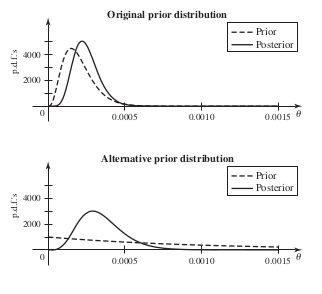
\includegraphics[width=0.5\textwidth]{img/7_2/img_1.png}

\end{figure}



\vspace{1cm}

É claro que a escolha da priori fará diferença com este pequeno conjunto de dados.
Os nomes ``a priori'' e ``a posteriori'' derivam das palavras latinas para ``anterior'' e ``posterior''. A distribuição a priori é a distribuição de $\theta$ que vem antes da observação dos dados, e a distribuição a posteriori vem depois da observação dos dados.

\subsection*{A Função de Verossimilhança}
O denominador no lado direito da Eq. (7.2.7) é simplesmente a integral do numerador sobre todos os valores possíveis de $\theta$. Embora o valor desta integral dependa dos valores observados $x_1, \dots, x_n$, ele não depende de $\theta$ e pode ser tratado como uma constante quando o lado direito da Eq. (7.2.7) é considerado como uma f.d.p. de $\theta$. Podemos, portanto, substituir a Eq. (7.2.7) pela seguinte relação:
\begin{equation}
\xi(\theta|\mathbf{x}) \propto f_n(\mathbf{x}|\theta)\xi(\theta). \tag{7.2.10}
\end{equation}
O símbolo de proporcionalidade $\propto$ é usado aqui para indicar que o lado esquerdo é igual ao lado direito, exceto possivelmente por um fator constante, cujo valor pode depender dos valores observados $x_1, \dots, x_n$, mas não depende de $\theta$. A constante apropriada que estabelecerá a igualdade dos dois lados na relação (7.2.10) pode ser determinada a qualquer momento usando o fato de que $\int_{\Omega} \xi(\theta|\mathbf{x})d\theta=1$, porque $\xi(\theta|\mathbf{x})$ é uma f.d.p. de $\theta$.
Uma das duas funções no lado direito da Eq. (7.2.10) é a f.d.p. a priori de $\theta$. A outra função também tem um nome especial.

\vspace{1cm}
\noindent\textbf{Definição 7.2.3} \quad \textbf{Função de Verossimilhança.} Quando a f.p. ou f.d.p. conjunta $f_n(\mathbf{x}|\theta)$ das observações em uma amostra aleatória é considerada como uma função de $\theta$ para valores dados de $x_1, \dots, x_n$, ela é chamada de \textit{função de verossimilhança}.

\vspace{1cm}
A relação (7.2.10) afirma que a f.d.p. a posteriori de $\theta$ é proporcional ao produto da função de verossimilhança e da f.d.p. a priori de $\theta$.
Usando a relação de proporcionalidade (7.2.10), muitas vezes é possível determinar a f.d.p. a posteriori de $\theta$ sem realizar explicitamente a integração em Eq. (7.2.6). Se pudermos reconhecer o lado direito da relação (7.2.10) como sendo, exceto por uma das f.d.p.s padrão introduzidas no Capítulo 5 ou em outro lugar neste livro, exceto possivelmente por um fator constante, então podemos facilmente determinar o fator apropriado que converterá o lado direito de (7.2.10) em uma f.d.p. adequada de $\theta$. Ilustraremos essas ideias considerando novamente o Exemplo 7.2.3.

\vspace{1cm}
\noindent\textbf{Exemplo 7.2.7} \quad \textbf{Proporção de Itens Defeituosos.} Suponha novamente, como no Exemplo 7.2.3, que a proporção $\theta$ de itens defeituosos em um grande lote manufaturado seja desconhecida e que a distribuição a priori de $\theta$ seja uma distribuição uniforme no intervalo $[0, 1]$. Suponha também que uma amostra aleatória de $n$ itens seja retirada do lote, e para $i=1, \dots, n$, seja $X_i=1$ se o i-ésimo item for defeituoso, e seja $X_i=0$ caso contrário. Então $X_1, \dots, X_n$ formam $n$ ensaios de Bernoulli com parâmetro $\theta$. Determinaremos a f.d.p. a posteriori de $\theta$.
Segue-se da Eq. (5.2.2) que a f.p. de cada observação $X_i$ é
$$ f(x|\theta) = 
\begin{cases}
\theta^x(1-\theta)^{1-x} & \text{para } x=0, 1, \\
0 & \text{caso contrário.}
\end{cases}
$$
Portanto, se seja $y=\sum_{i=1}^{n}x_i$, então a f.p. conjunta de $X_1, \dots, X_n$ pode ser escrita na seguinte forma para $x_i=0$ ou $1 \, (i=1, \dots, n)$:
\begin{equation}
f_n(\mathbf{x}|\theta) = \theta^y(1-\theta)^{n-y}. \tag{7.2.11}
\end{equation}
Uma vez que a f.d.p. a priori $\xi(\theta)$ é dada por Eq. (7.2.1), segue-se que para $0 < \theta < 1$,
\begin{equation}
f_n(\mathbf{x}|\theta)\xi(\theta) = \theta^y(1-\theta)^{n-y}. \tag{7.2.12}
\end{equation}
Quando comparamos esta expressão com Eq. (5.8.3), podemos ver que, exceto por um fator constante, é a f.d.p. da distribuição beta com parâmetros $\alpha = y+1$ e $\beta = n-y+1$. Uma vez que a f.d.p. a posteriori $\xi(\theta|\mathbf{x})$ é proporcional ao lado direito da Eq. (7.2.12), segue-se que $\xi(\theta|\mathbf{x})$ deve ser a f.d.p. da distribuição beta com parâmetros $a=y+1$ e $b=n-y+1$. Portanto, para $0 < \theta < 1$,
\begin{equation}
\xi(\theta|\mathbf{x}) = \frac{\Gamma(n+2)}{\Gamma(y+1)\Gamma(n-y+1)}\theta^y(1-\theta)^{n-y}. \tag{7.2.13}
\end{equation}
Neste exemplo, a estatística $Y = \sum_{i=1}^{n}X_i$ está sendo usada para construir a distribuição a posteriori, e, portanto, será usada em qualquer inferência que se baseie na distribuição a posteriori.

\vspace{1cm}
\noindent\textbf{Nota: Constante de Normalização para f.d.p. a Posteriori.} Os passos que nos levaram de (7.2.12) para (7.2.13) são um exemplo de uma técnica muito comum para determinar uma f.d.p. a posteriori. Pode-se extrair qualquer fator constante inconveniente da f.p. ou f.d.p. a priori e da função de verossimilhança antes de multiplicá-los juntos como em (7.2.10). Então, olhamos para o produto resultante, chame-o de $g(\theta)$, para ver se o reconhecemos como se parecendo com parte de uma f.d.p. que já vimos. Se, de fato, encontrarmos uma f.d.p. nomeada com a qual estamos familiarizados que seja igual a $cg(\theta)$, então nossa f.d.p. a posteriori também é $cg(\theta)$, e nossa distribuição a posteriori tem o nome correspondente, assim como no Exemplo 7.2.7.

\subsection*{Observações Sequenciais e Previsão}
Em muitos experimentos, as observações $X_1, \dots, X_n$, que formam a amostra aleatória, devem ser obtidas sequencialmente, ou seja, uma de cada vez. Em tal experimento, o valor de $X_1$ é observado primeiro, o valor de $X_2$ é observado em seguida, o valor de $X_3$ é então observado, e assim por diante. Suponha que a f.d.p. a posteriori do parâmetro $\theta$ após o valor de $x_1$ ter sido observado, possa ser calculada da maneira usual a partir da relação
\begin{equation}
\xi(\theta|x_1) \propto f(x_1|\theta)\xi(\theta). \tag{7.2.14}
\end{equation}
Como $X_1$ e $X_2$ são condicionalmente independentes dado $\theta$, a f.p. ou f.d.p. condicional de $X_2$ dado $\theta$ e $X_1=x_1$ é a mesma que dado $\theta$ apenas, a saber, $f(x_2|\theta)$. Portanto, a f.d.p. a posteriori de $\theta$ na Eq. (7.2.14) serve como a f.d.p. a priori de $\theta$ quando o valor de $X_2$ está para ser observado. Assim, após o valor de $x_2$ ter sido observado, a f.d.p. a posteriori de $\theta$ pode ser calculada a partir da relação
\begin{equation}
\xi(\theta|x_1, x_2) \propto f(x_2|\theta)\xi(\theta|x_1). \tag{7.2.15}
\end{equation}
Podemos continuar desta forma, calculando uma f.d.p. a posteriori atualizada de $\theta$ após cada observação e usando essa f.d.p. como a f.d.p. a priori de $\theta$ para a próxima observação. A f.d.p. a posteriori $\xi(\theta|x_1, \dots, x_{n-1})$ após os valores $x_1, \dots, x_{n-1}$ terem sido observados, será em última análise a f.d.p. a priori de $\theta$ para o valor final observado $x_n$. A f.d.p. a posteriori após todos os $n$ valores $x_1, \dots, x_n$ terem sido observados, será, portanto, especificada pela relação
\begin{equation}
\xi(\theta|x_1, \dots, x_n) \propto f(x_n|\theta)\xi(\theta|x_1, \dots, x_{n-1}). \tag{7.2.16}
\end{equation}
Alternativamente, depois de todos os $n$ valores $x_1, \dots, x_n$ terem sido observados, poderíamos calcular a f.d.p. a posteriori de $\theta$ da maneira usual, combinando a f.d.p. ou f.p. conjunta $f_n(\mathbf{x}|\theta)$ com a f.d.p. a priori original $\xi(\theta)$, como indicado em Eq. (7.2.7). Pode ser mostrado (ver Exercício 8) que a f.d.p. a posteriori $\xi(\theta|\mathbf{x})$ será a mesma, independentemente de ser calculada diretamente usando Eq. (7.2.7) ou sequencialmente usando Eqs. (7.2.14), (7.2.15) e (7.2.16). Esta propriedade foi ilustrada na Seção 2.3 (ver página 80) para uma moeda que se sabe ser justa ou ter cara em ambos os lados. Após cada lançamento da moeda, a probabilidade a posteriori de a moeda ser justa é atualizada.
As constantes de proporcionalidade nas Eqs. (7.2.14)-(7.2.16) têm uma interpretação útil. Por exemplo, em (7.2.16) a constante de proporcionalidade é 1 sobre a integral do lado direito com respeito a $\theta$. Mas esta integral é a f.d.p. ou f.p. condicional de $X_n$ dado $X_1=x_1, \dots, X_{n-1}=x_{n-1}$ de acordo com a versão condicional da lei da probabilidade total (3.7.16). Por exemplo, se $\theta$ tem uma distribuição contínua,
\begin{equation}
f(x_n|x_1, \dots, x_{n-1}) = \int f(x_n|\theta)\xi(\theta|x_1, \dots, x_{n-1})d\theta. \tag{7.2.17}
\end{equation}
Se estivermos interessados em prever a n-ésima observação após observar as primeiras $n-1$, podemos usar (7.2.17), que também é 1 sobre a constante de proporcionalidade em Eq. (7.2.16), como a f.d.p. ou f.p. condicional de $X_n$ dados os primeiros $n-1$ observáveis.

\vspace{1cm}
\noindent\textbf{Exemplo 7.2.8} \quad \textbf{Tempo de Vida de Lâmpadas Fluorescentes.} No Exemplo 7.2.6, condicional a $\theta$, os tempos de vida de lâmpadas fluorescentes são variáveis aleatórias exponenciais independentes com parâmetro $\theta$. Também observamos os tempos de vida de cinco lâmpadas, e a distribuição a posteriori de $\theta$ foi encontrada como sendo a distribuição gama com parâmetros 9 e 36.178. Suponha que queiramos prever o tempo de vida $X_6$ da próxima lâmpada.
A f.d.p. condicional de $X_6$, o tempo de vida da próxima lâmpada, dadas as primeiras cinco vidas, integra o produto de $\xi(\theta|\mathbf{x})$ e $f(x_6|\theta)$ em relação a $\theta$. A f.d.p. a posteriori de $\theta$ é $\xi(\theta|\mathbf{x}) = 2.633 \times 10^{36} \theta^8 e^{-36.178\theta}$ para $\theta > 0$. Então, para $x_6 > 0$
\begin{align}
f(x_6|\mathbf{x}) &= \int_0^{\infty} 2.633 \times 10^{36} \theta^8 e^{-36.178\theta} \theta e^{-x_6\theta} d\theta \nonumber \\
&= 2.633 \times 10^{36} \int_0^{\infty} \theta^9 e^{-(x_6+36.178)\theta} d\theta \tag{7.2.18} \\
&= 2.633 \times 10^{36} \frac{\Gamma(10)}{(x_6+36.178)^{10}} = \frac{9.555 \times 10^{41}}{(x_6+36.178)^{10}}. \nonumber
\end{align}
Podemos usar esta f.d.p. para realizar qualquer cálculo que desejarmos sobre a distribuição de $X_6$ dados os tempos de vida observados. Por exemplo, a probabilidade de que a sexta lâmpada dure mais de 3000 horas é igual a
$$ \Pr(X_6>3000|\mathbf{x}) = \int_{3000}^{\infty} \frac{9.555 \times 10^{41}}{9 \times 39.178^9} dx_6 = \frac{9.555 \times 10^{41}}{9 \times 39.178^9} = 0.4882. $$
Podemos continuar a análise de sensibilidade que foi iniciada no Exemplo 7.2.6. É importante saber a probabilidade de que o próximo tempo de vida seja de pelo menos 3000, podemos ver quanta influência a escolha da distribuição a priori teve nesta computação. Usando a segunda distribuição a priori (gama com parâmetros 1 e 1000), descobrimos que a distribuição a posteriori de $\theta$ era a gama com parâmetros 6 e 17.178. Poderíamos calcular a f.d.p. condicional de $X_6$ dados os dados observados da mesma forma que fizemos com a priori original, e seria
\begin{equation}
f(x_6|\mathbf{x}) = \frac{1.542 \times 10^{26}}{(x_6+17.178)^7}, \quad \text{para } x_6 > 0. \tag{7.2.19}
\end{equation}
Com esta f.d.p., a probabilidade de que $X_6 > 3000$ é
$$ \Pr(X_6>3000|\mathbf{x}) = \int_{3000}^{\infty} \frac{1.542 \times 10^{26}}{(x_6+17.178)^7} dx_6 = \frac{1.542 \times 10^{26}}{6 \times 20.178^6} = 0.3807. $$

\vspace{1cm}

\begin{figure}[H]

\centering

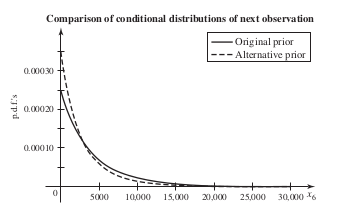
\includegraphics[width=0.5\textwidth]{img/7_2/img_2.png}


\end{figure}
\vspace{1cm}

Como notamos no final do Exemplo 7.2.6, as diferentes prioris fazem uma diferença considerável nas inferências que podemos fazer. É importante ter um valor preciso de $\Pr(X_6 > 3000|\mathbf{x})$, precisamos de uma amostra maior. Os dois f.d.p.s diferentes de $X_6$ podem ser comparados na Fig. 7.2. A f.d.p. de Eq. (7.2.18) é maior para valores intermediários de $x_6$, enquanto a de Eq. (7.2.19) é maior para os valores extremos de $x_6$.

\subsection*{Resumo}
A distribuição a priori de um parâmetro descreve nossa incerteza sobre o parâmetro antes de observar quaisquer dados. A função de verossimilhança é a f.d.p. ou f.p. condicional dos dados, considerada como uma função do parâmetro dados os dados. A verossimilhança nos diz o quanto os dados alteram nossa incerteza. Valores grandes da verossimilhança corresponderão a valores de parâmetro onde a posteriori será maior do que a priori. Valores baixos da verossimilhança ocorrerão em valores de parâmetro onde a posteriori será menor do que a priori. A distribuição a posteriori do parâmetro é a distribuição condicional do parâmetro dados os dados. Ela é obtida usando o teorema de Bayes para variáveis aleatórias, que vimos pela primeira vez na página 148. Podemos prever observações futuras que são condicionalmente independentes dos dados observados dado $\theta$ usando a versão condicional da lei da probabilidade total que vimos na página 163.

\section*{Exercícios}
\begin{enumerate}
    \item Considere novamente a situação descrita no Exemplo 7.2.8. Desta vez, suponha que o experimentador acredite que a distribuição a priori de $\theta$ é a distribuição gama com parâmetros 1 e 5000. Que valor o experimentador calcularia para $\Pr(X_6 > 3000|\mathbf{x})$?

    \item Suponha que a proporção $\theta$ de itens defeituosos em um grande lote manufaturado seja 0,1 ou 0,2, e que a f.p. (função de probabilidade) a priori de $\theta$ seja a seguinte:
    $$ \xi(0.1) = 0.7 \quad \text{e} \quad \xi(0.2) = 0.3. $$
    Suponha também que, quando oito itens são selecionados aleatoriamente do lote, descobre-se que exatamente dois deles são defeituosos. Determine a f.p. a posteriori de $\theta$.

    \item Suponha que o número de defeitos em um rolo de fita de gravação magnética tenha uma distribuição de Poisson para a qual a média $\lambda$ é 1,0 ou 1,5, e a f.p. a priori de $\lambda$ é a seguinte:
    $$ \xi(1.0) = 0.4 \quad \text{e} \quad \xi(1.5) = 0.6. $$
    Se um rolo de fita selecionado aleatoriamente apresentar três defeitos, qual é a f.p. a posteriori de $\lambda$?

    \item Suponha que a distribuição a priori de algum parâmetro $\theta$ seja uma distribuição gama para a qual a média é 10 e a variância é 5. Determine a f.d.p. (função de densidade de probabilidade) a priori de $\theta$.

    \item Suponha que a distribuição a priori de algum parâmetro $\theta$ seja uma distribuição beta para a qual a média é 1/3 e a variância é 1/45. Determine a f.d.p. a priori de $\theta$.

    \item Suponha que a proporção $\theta$ de itens defeituosos em um grande lote manufaturado seja desconhecida, e a distribuição a priori de $\theta$ seja a distribuição uniforme no intervalo $[0, 1]$. Quando oito itens são selecionados aleatoriamente do lote, descobre-se que exatamente três deles são defeituosos. Determine a distribuição a posteriori de $\theta$.

    \item Considere novamente o problema descrito no Exercício 6, mas suponha agora que a f.d.p. a priori de $\theta$ seja a seguinte:
    $$ \xi(\theta) = 
    \begin{cases}
        2(1-\theta) & \text{para } 0 < \theta < 1, \\
        0 & \text{caso contrário.}
    \end{cases}
    $$
    Como no Exercício 6, suponha que em uma amostra aleatória de oito itens, exatamente três sejam defeituosos. Determine a distribuição a posteriori de $\theta$.

    \item Suponha que $X_1, \dots, X_n$ formem uma amostra aleatória de uma distribuição para a qual a f.d.p. é $f(x|\theta)$, o valor de $\theta$ é desconhecido, e a f.d.p. a priori de $\theta$ é $\xi(\theta)$. Mostre que a f.d.p. a posteriori $\xi(\theta|\mathbf{x})$ é a mesma, quer seja calculada diretamente usando a Eq. (7.2.7) ou sequencialmente usando as Eqs. (7.2.14), (7.2.15) e (7.2.16).

    \item Considere novamente o problema descrito no Exercício 6, e assuma a mesma distribuição a priori de $\theta$. Suponha, no entanto, que em vez de selecionar uma amostra aleatória de oito itens do lote, realizemos o seguinte experimento: os itens do lote são selecionados aleatoriamente um a um até que exatamente três defeituosos tenham sido encontrados. Se descobrirmos que devemos selecionar um total de oito itens neste processo, qual é a distribuição a posteriori de $\theta$ no final do experimento?
    
    \item Suponha que uma única observação $X$ deva ser retirada da distribuição uniforme no intervalo $[\theta - \frac{1}{2}, \theta + \frac{1}{2}]$, o valor de $\theta$ é desconhecido, e a distribuição a priori de $\theta$ é a distribuição uniforme no intervalo $[10, 20]$. Se o valor observado de $X$ for 12, qual é a distribuição a posteriori de $\theta$?
    
    \item Considere novamente as condições do Exercício 10, e assuma a mesma distribuição a priori de $\theta$. Suponha, no entanto, que seis observações sejam selecionadas aleatoriamente da distribuição uniforme no intervalo $[\theta - \frac{1}{2}, \theta + \frac{1}{2}]$, e seus valores sejam 11.0, 11.5, 11.7, 11.1, 11.4 e 10.9. Determine a distribuição a posteriori de $\theta$.
\end{enumerate}